%!TEX root = thesis.tex
\chapter{Cache Oriented Obfuscation on the System without Coherence}

In this chapter of the thesis, we proposed a method to design a reliable and efficient obfuscation technique for tightly coupled multi-processing systems by exploiting the feature of cache oriented programming. Besides, we emphasized a number of points to characterize proper attack vector. After we had elaborated our obfuscation methods and its primitives, we discussed what it is and what it is not on pitfalls and fallacies section. Finally, on the implementation section, we drew a picture of possibilities on practical applications. However, this chapter and this thesis does not concern specific and deeper studies on obfuscation and memory protection(TLB, MMU, MPU). They are correlated with our thesis, but it is on the upper layer which is like TCP and IP layers of network. On the whole and in the brief, this chapter gives an isolated workspace for obfuscation techniques.

As we mentioned previous chapters, malware detection tools needs sensors to analysis running code. Regular sensors observes real-time systems with monitoring shared memory, it means a lot for operating systems, because OS, computer architecture and computer conventions assume everything on the memory and ultimate and consistent. With this assumption, dumping memory and analysing snapshots are practically efficient and convenient way of malware monitoring and detecting. There are actually a number of sensor type for real time memory observation: external monitors, internal monitors, and exotically virtual monitoring. External monitors in contrast with internal monitors are the systems which is comprised with external hardware devices and its software component. They could be implemented on external PCI or GPU devices, FPGA co-processor or on-board chip\cite{Christos2013}. They are efficient because they are pre-installed, omnipresent systems which does not require OS and other middleware platform which constrains their limits. Also They are efficient because they are the hardwares which can be designed with the purpose. However, they are expensive to implement comparing with internal monitors. Internal monitors are using regular devices on the computer architecture such as CPU, and they are working under the operating systems' kernel, which could be easy to deceive \cite{Adnan2011}, \cite{rutkowska2006rootkits}. Our methods is actually not depending on the monitoring type, since it is related with where they are monitoring.

Tightly coupled multi-processing systems have many processor with their own caches and one shared memory\cite{Jim2007}. Cache memories are not developed with same purpose of memories, but are developed for performance reason which we discussed in background studies. If we exploit them and design our program properly, cache memories could be used as another layer of memories, and on the monitoring side, even if it perfectly scan and detect memories, cache memories are still out of the box.

The required systems for our technique in this chapter is tightly coupled multi-processing systems without cache coherence interconnector. Also, we need simple Harvard computer architecture instead of Von Neumann. Incoherent systems are surprisingly popular because of the implementation errors i.e. Samsung's mainstream CPU Exynos 5410 which sold millions, and also due to costs. Many hardware designers also believe programming with shared memory is not appropriate way and platforms such as Android already using message based communication on multi-threaded application, and  they implement clustered processors which limits programs instead of implementing expensive coherency interconnector. Yet they do not consider security approaches.
    \begin{figure}[h!]
        \centering
        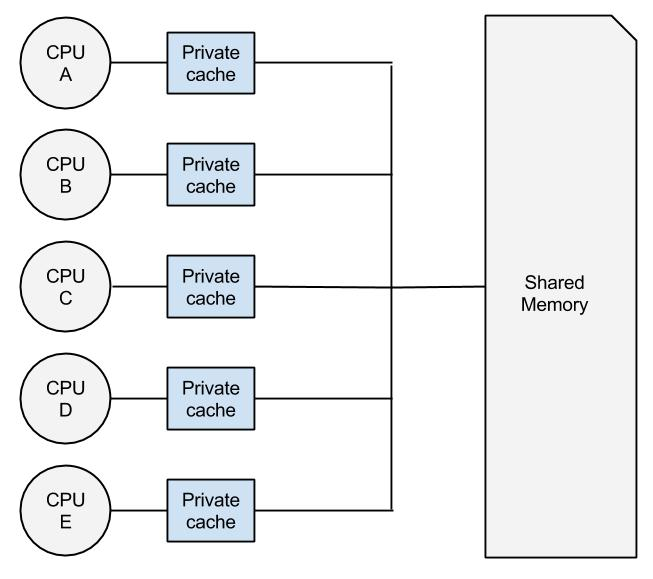
\includegraphics[width=1\textwidth]{img/Tightly Coupled Multi-Processing Systems.jpg}
        \caption{An Example of Tightly Coupled Multi-Processing Systems}
        \label{fig:tightlycoupled}
    \end{figure}
	

	\section{Exploiting Tightly Coupled Multi-Processing Systems}
	    \begin{figure}[h!]
	        \centering
	        \includegraphics[width=1\textwidth]{img/attack vector.jpg}
	        \caption{Attack vector flow chart}
	        \label{fig:atackvector}
	    \end{figure}
	    \subsection{Reconnaissance and Design}
	    \subsection{Setting system up and Loading Cache Memory}
	    \begin{lstlisting}
	mov r2, 0x012345 #address
	mov r3, 0x013456 #end of gadget
	mov r4, 0 #counter
fetch: 	addi r2, r4 # add size of word to address
	mov r1, [r2] #Load address from memory
	cmp r2,r3 # compare r2 and r3
	jl fetch
\end{lstlisting}

	    \subsection{Obfuscating Running and Deobfuscating gadget}
	    \subsection{Regeneration}
	\section{Pitfalls and Fallacies}
			Coherency Mechanism
			Harvard Arch
			Caches are not memory
			Context switching

